\documentclass[11pt, a4paper]{article}

\usepackage[margin=1in]{geometry}
\usepackage{graphicx}
\usepackage{booktabs}
\usepackage{amsmath}
\usepackage{amssymb}
\usepackage{hyperref}
\usepackage{titlesec}

\titleformat{\section}{\large\bfseries}{\thesection}{1em}{}
\titleformat{\subsection}{\normalsize\bfseries}{\thesubsection}{1em}{}

\graphicspath{{../Overall_Report/figures/}{../Problems_Report/figures/}}

\title{\textbf{Copy-Paste Augmentation Report for MinneApple and Global Wheat Head}}
\author{}

\begin{document}

\maketitle

\section{Objective}
This report aims to show my analysis and thinking about why detection performance decreases when using copy-paste augmentation.

\section{Recap}
\begin{itemize}
\item \textbf{Scoring system:} the score is meant to measure how hard each object and image is for the detector. For an object $g$, we use low-confidence predictions and compute

Let $G(I)$ be the set of ground-truth objects in image $I$, and let $\mathcal{P}$ be the set of model predictions. For a ground-truth object $g$ denote by
\[\mathcal{P}(g;\tau)\;=\;\{\;p\in\mathcal{P}:\;\mathrm{IoU}(p,g)\ge\tau\;\}\]
the subset of predictions whose intersection-over-union with $g$ exceeds the IoU threshold $\tau\in[0,1]$. Each prediction $p$ has a confidence $\mathrm{conf}(p)\in[0,1]$ and an IoU value $\mathrm{IoU}(p,g)\in[0,1]$.

For $\alpha,\beta\ge0$ we define the object difficulty score
\[
S_{\mathrm{obj}}(g)
=
\begin{cases}
\displaystyle\min_{p\in\mathcal{P}(g;\tau)}\left[\alpha\bigl(1-\mathrm{conf}(p)\bigr)+\beta\bigl(1-\mathrm{IoU}(p,g)\bigr)\right], & \mathcal{P}(g;\tau)\neq\varnothing, \\
\alpha+\beta, & \mathcal{P}(g;\tau)=\varnothing.
\end{cases}
\]

This definition has the following properties:
\begin{itemize}
\item Lower confidence or lower IoU increases the score (more difficult). 
\item The upper bound for $S_{\mathrm{obj}}(g)$ is $\alpha+\beta$ (occurs when no matching prediction exists). 
\end{itemize}

The image-level difficulty score aggregates object difficulties and penalizes false positives. 

With aggregation weights $w_1,w_2\ge0$, we define:
\[
S_{\mathrm{img}}(I)=w_1\cdot\frac{1}{|G(I)|}\sum_{g\in G(I)}S_{\mathrm{obj}}(g)\;+
\;w_2\cdot\mathrm{FP\ rate}(I;\gamma,\tau).
\]

Interpretation: higher $S_{\mathrm{img}}(I)$ indicates that the image contains harder-to-detect objects and/or a larger proportion of false positives.

\item \textbf{Copy-paste pipeline:} we use this because we believe increasing the appearance of objects and backgrounds can improve performance in agricultural detection problems.
\begin{enumerate}
\item Select a background image.
\item Select one or more objects to paste.
\item Determine how many objects to paste (2-8 objects).
\item Apply geometry transformations (scaling and rotation) on selected objects.
\item Paste objects and generate new labels.
\end{enumerate}
\end{itemize}

\section{Experiments}
We ran two experiments to compare detection results under baseline, random copy-paste, and score-guided copy-paste.

The same pipeline was used across seeds 123, 456, and 789, detail can be see in Table \ref{tab:augmentation_config}: dataset ratio 0.3, 2--5 pasted objects per image, scale jitter within $\pm 20\%$, rotation within $\pm 15^\circ$, overlap avoidance enabled, and only the selection policy changed between random and score-guided sampling.

\subsection{MinneApple results}
\begin{table}[htbp]
\centering
\small
\setlength{\tabcolsep}{4pt}
\caption{MinneApple: 3-seed mean COCO AP on the original test set}
\label{tab:minneapple_results}
\begin{tabular}{lrrrrrr}
\toprule
Condition & AP & AP50 & AP75 & AP$_S$ & AP$_M$ & AP$_L$ \\
\midrule
Baseline & 0.439 & 0.771 & 0.452 & 0.300 & 0.592 & 0.645 \\
Random CP & 0.415 & 0.741 & 0.427 & 0.279 & 0.563 & 0.669 \\
\textbf{Score CP} & \textbf{0.428} & \textbf{0.759} & \textbf{0.440} & \textbf{0.286} & \textbf{0.581} & \textbf{0.637} \\
\bottomrule
\end{tabular}%
\end{table}

\begin{itemize}
\item MinneApple is the only case where score-guided copy-paste is clearly better than random copy-paste, but the improvement is still not enough to recover the baseline.
\item  Score CP improves AP, AP50, AP75, and especially AP$_S$ and AP$_M$ relative to Random CP, indicating the score pushes selection toward smaller and medium objects.
\item  Both augmentation variants still reduce performance compared with the baseline; the gain is only relative, not absolute.
\end{itemize}

\subsection{Global Wheat Head results}
\begin{table}[htbp]
\centering
\small
\setlength{\tabcolsep}{4pt}
\caption{Global Wheat Head: 3-seed mean COCO AP on the original test set}
\label{tab:gwhd_results}
\begin{tabular}{lrrrrrr}
\toprule
Condition & AP & AP50 & AP75 & AP$_S$ & AP$_M$ & AP$_L$ \\
\midrule
Baseline & 0.507 & 0.922 & 0.491 & 0.136 & 0.501 & 0.550 \\
Random CP & 0.486 & 0.905 & 0.456 & 0.118 & 0.480 & 0.529 \\
\textbf{Score CP} & \textbf{0.484} & \textbf{0.905} & \textbf{0.455} & \textbf{0.098} & \textbf{0.477} & \textbf{0.531} \\
\bottomrule
\end{tabular}%
\end{table}

\begin{itemize}
\item  Global Wheat Head shows the same failure pattern, with even less separation between random and score-guided selection.
\item  Both copy-paste variants remain below baseline on every main metric; Score CP is only marginally different from Random CP.
\item  The gap is too small to support a meaningful claim of improvement; this appears to be augmentation noise rather than a useful intervention.
\end{itemize}

\section{Analysis and Hypotheses}

\subsection{MinneApple}
\begin{itemize}
\item \textbf{Observation:} The augmented examples still look somewhat artificial, even though the pasted objects are visually plausible (see Appendix Figures~\ref{fig:minneapple_aug_vs_ori} and~\ref{fig:minneapple_object_paste}). Moreover, in the feature-space view, the initial training distribution is already quite far from the test distribution, and the augmented data does not clearly move it closer (see Appendix Figure~\ref{fig:minneapple_feature_space}).
\item \textbf{Analysis:} The feature-space and object-paste views suggest that the augmentation is changing the training distribution without clearly moving it toward the test distribution (see Appendix Figures~\ref{fig:minneapple_feature_space} and~\ref{fig:minneapple_object_paste}). 
\item \textbf{Hypothesis:} The performance drop comes from pasted-object noise and from augmented images that are not close enough to the test distribution.
\end{itemize}

\subsection{Global Wheat Head}
\begin{itemize}
\item \textbf{Observation:} Score-guided sampling concentrates pasted objects in a narrower portion of the source domains, especially the arvalis domains (see Appendix Figure~\ref{fig:gwhd_add_augmentation}).
\item \textbf{Analysis:} This concentration does not improve detection, and the feature-space plus AP views still indicate a mismatch with test performance (see Appendix Figures~\ref{fig:gwhd_feature_space} and~\ref{fig:gwhd_ap_result}).
\item \textbf{Hypothesis:} GWHD is dominated by domain shift, so copy-paste alone is unlikely to solve the real problem. The question of why score-guiided new augmentation image make it far differnt from the original set in the embeddig space is still open.
\end{itemize}

\section{Conclusion}
\begin{itemize}
\item On MinneApple, score-guided copy-paste is better than random copy-paste, especially for small and medium objects, but both still underperform the baseline. 
\item On Global Wheat Head, random and score-guided sampling are almost the same, and both remain below baseline. Overall, the evidence suggests that copy-paste adds noise and does not reliably move the training data toward the test distribution. For GWHD, the failure mode looks too much like domain shift to be solved by copy-paste alone.
\item 
\end{itemize}

\appendix
\section{Appendix: Additional Figures and Details}

\begin{figure}[htbp]
\centering
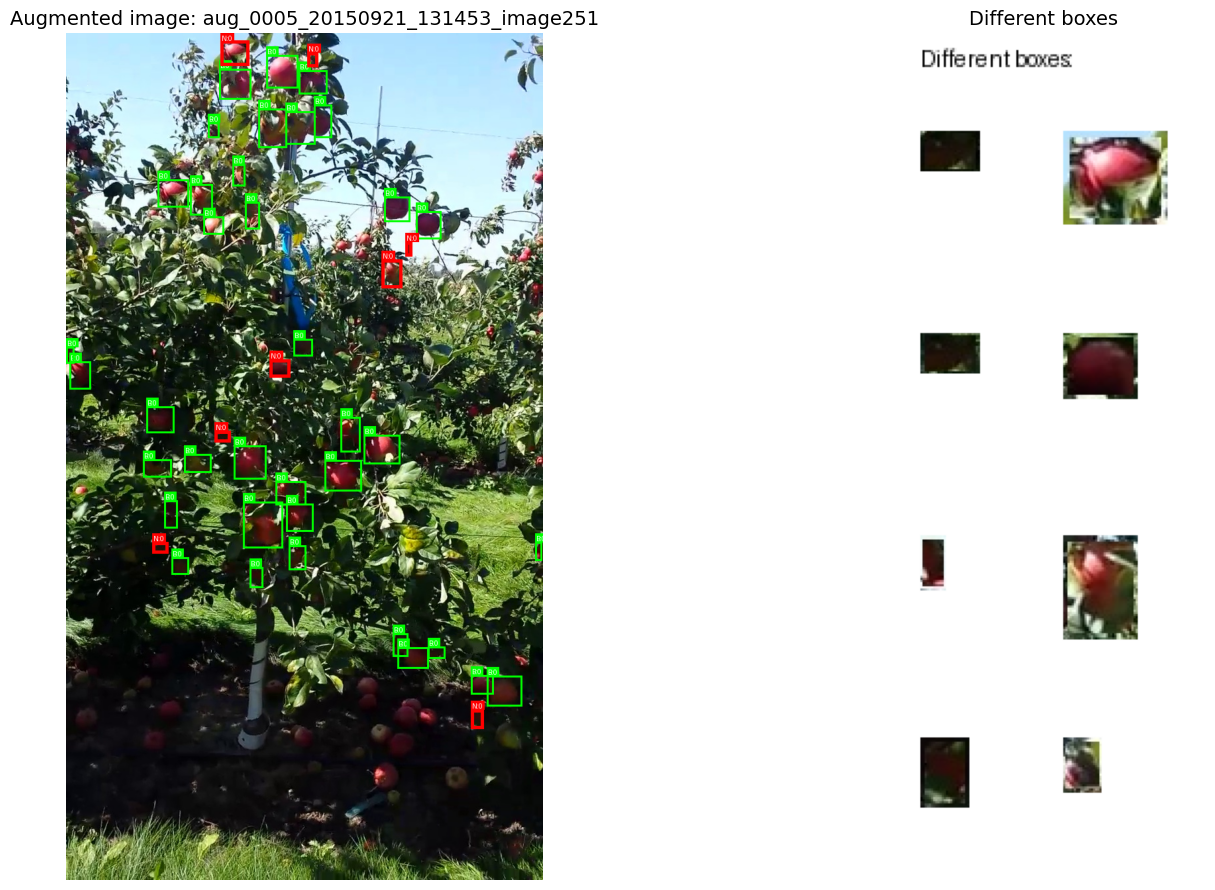
\includegraphics[width=0.92\linewidth,height=0.33\textheight,keepaspectratio]{aug_vs_origin.png}
\caption{MinneApple: augmented vs. original examples.}
\label{fig:minneapple_aug_vs_ori}
\end{figure}

\begin{figure}[htbp]
\centering
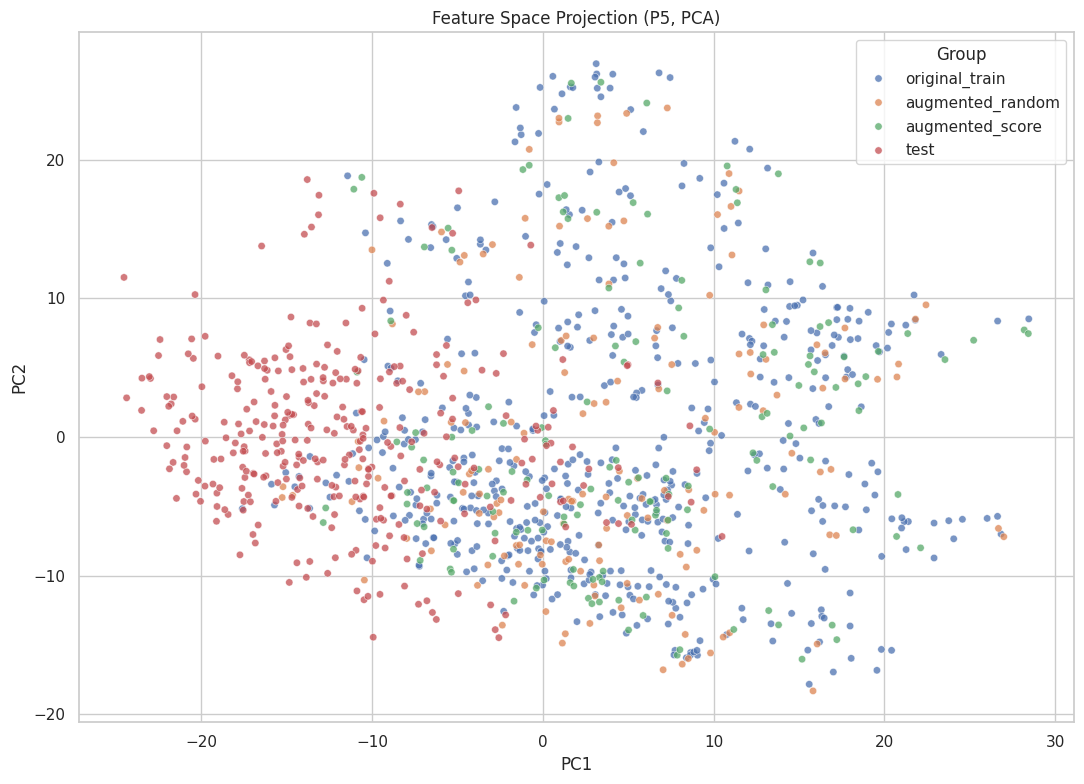
\includegraphics[width=0.92\linewidth,height=0.33\textheight,keepaspectratio]{mineapple_feature_space.png}
\caption{MinneApple: feature-space projection.}
\label{fig:minneapple_feature_space}
\end{figure}

\begin{figure}[htbp]
\centering
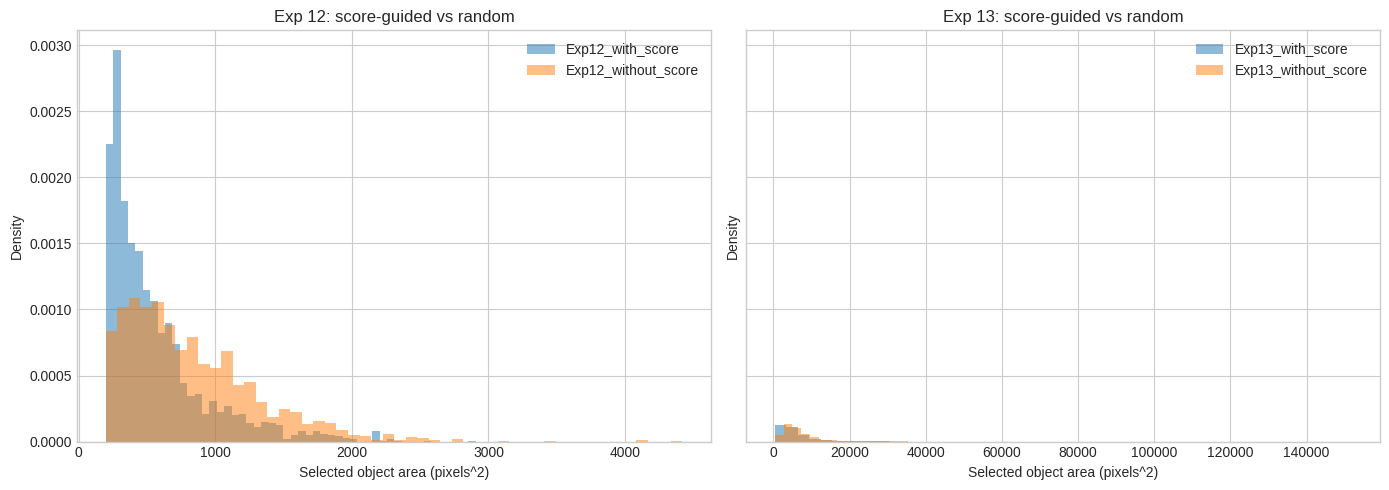
\includegraphics[width=0.92\linewidth,height=0.33\textheight,keepaspectratio]{mineapple_object_paste_analysis.png}
\caption{MinneApple: object-paste analysis.}
\label{fig:minneapple_object_paste}
\end{figure}

\begin{figure}[htbp]
\centering
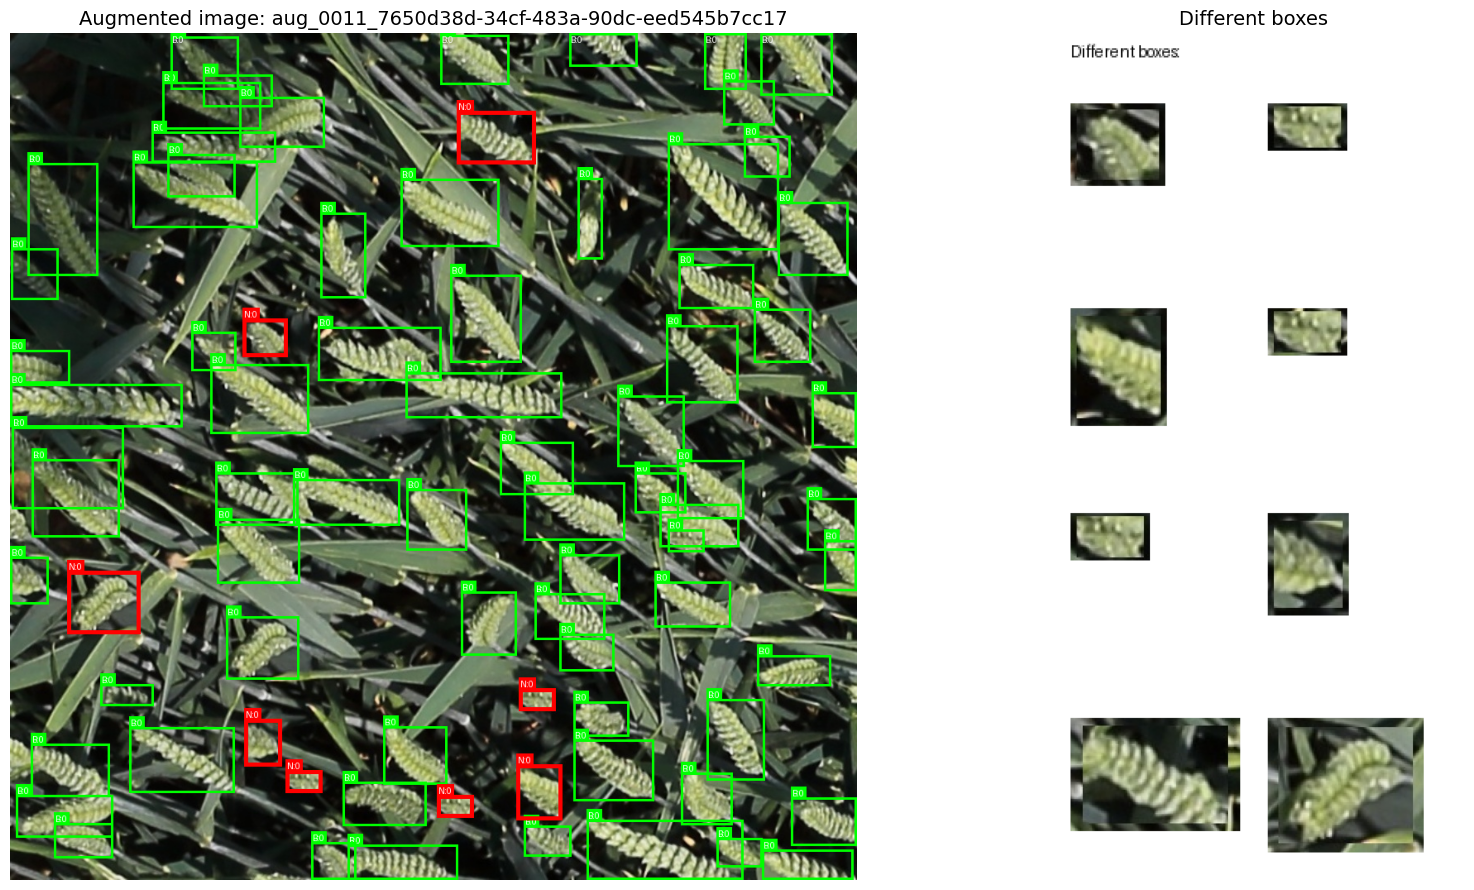
\includegraphics[width=0.92\linewidth,height=0.33\textheight,keepaspectratio]{gwhd_augvsori.png}
\caption{Global Wheat Head: augmented vs. original examples.}
\label{fig:gwhd_aug_vs_ori}
\end{figure}

\begin{figure}[htbp]
\centering
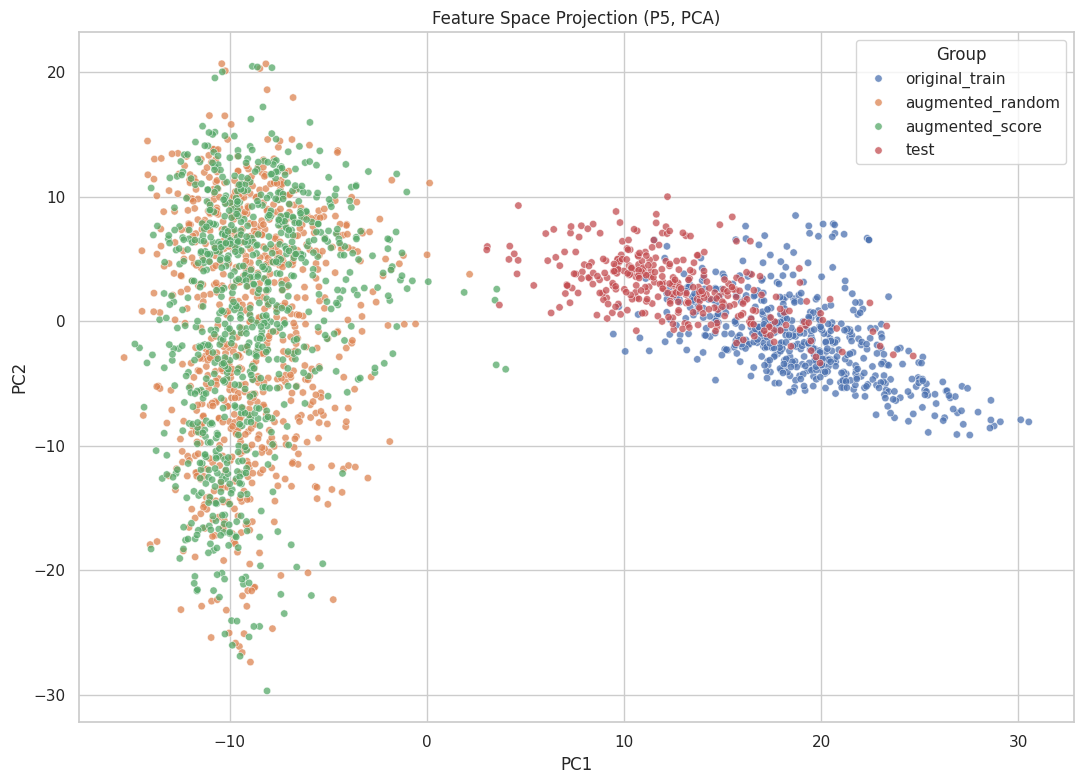
\includegraphics[width=0.92\linewidth,height=0.33\textheight,keepaspectratio]{gwhd_feature_space.png}
\caption{Global Wheat Head: feature-space projection.}
\label{fig:gwhd_feature_space}
\end{figure}

\begin{figure}[htbp]
\centering
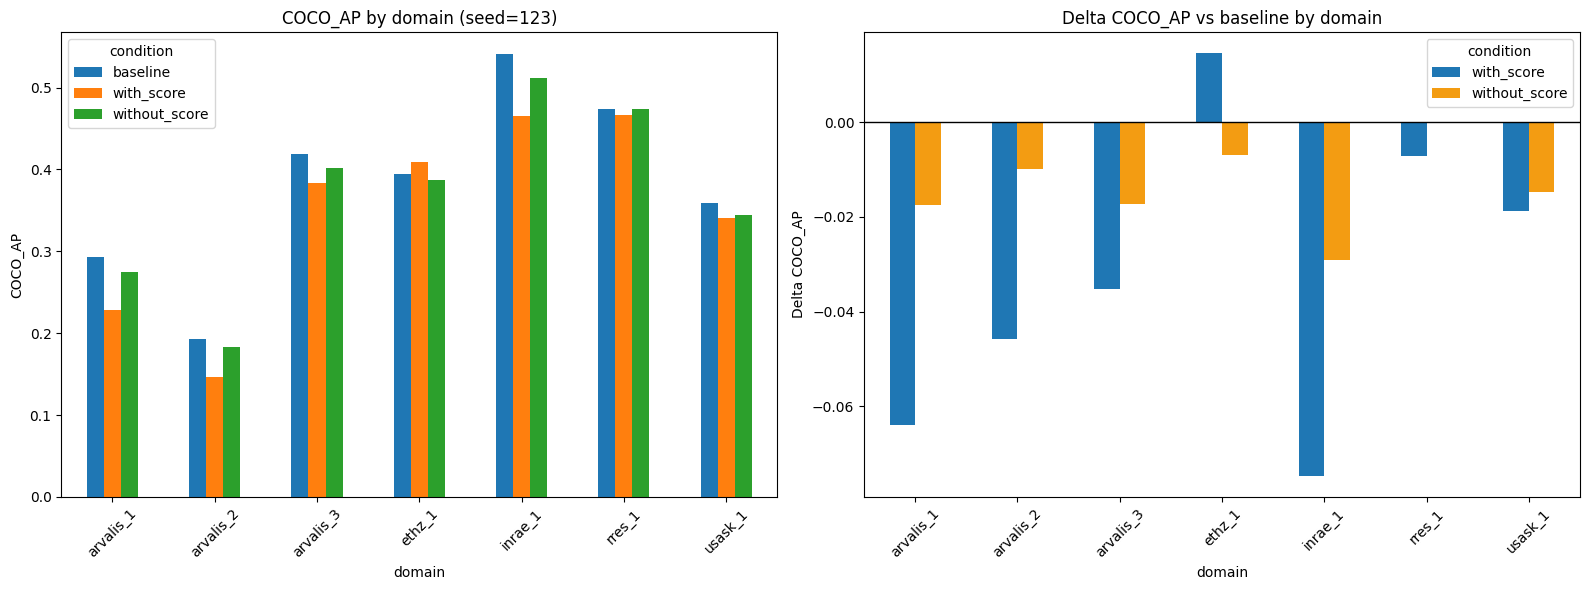
\includegraphics[width=0.92\linewidth,height=0.33\textheight,keepaspectratio]{gwhd_ap_result.png}
\caption{Global Wheat Head: AP comparison result.}
\label{fig:gwhd_ap_result}
\end{figure}

\begin{figure}[htbp]
\centering
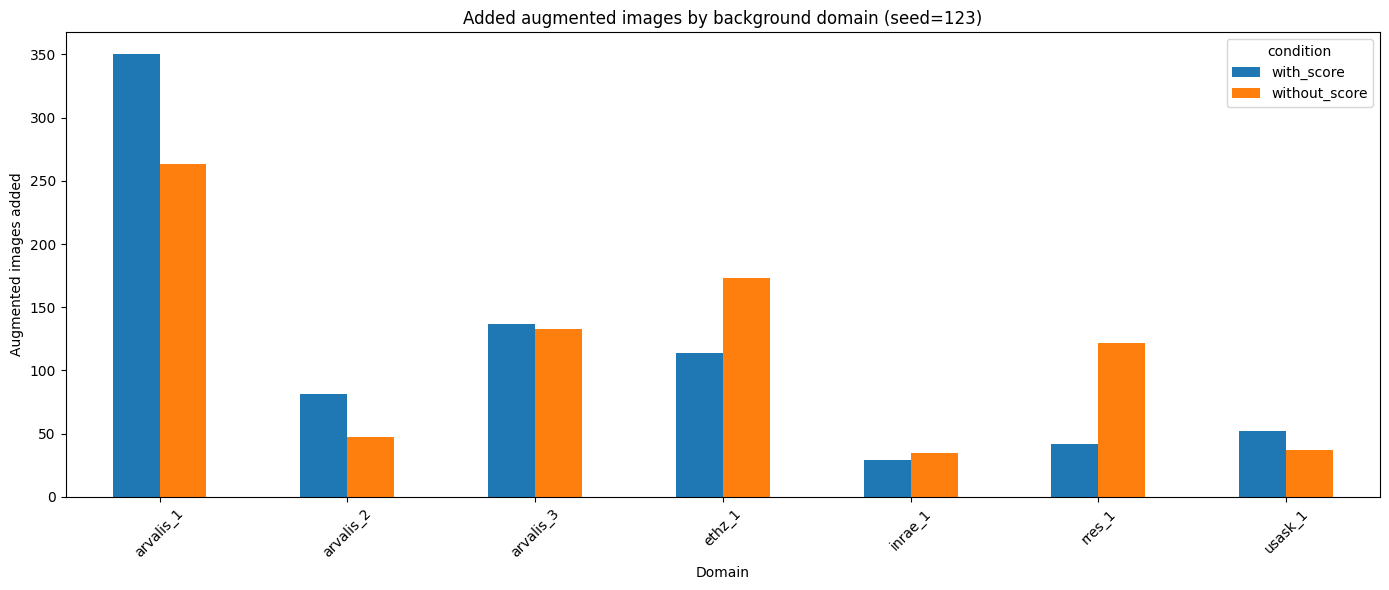
\includegraphics[width=0.92\linewidth,height=0.33\textheight,keepaspectratio]{add_augmentation.png}
\caption{Global Wheat Head: added augmentation distribution.}
\label{fig:gwhd_add_augmentation}
\end{figure}

\subsection{Configuration Tables}

\begin{table}[htbp]
\centering
\small
\setlength{\tabcolsep}{6pt}
\caption{Training configuration (MinneApple vs Global Wheat Head)}
\label{tab:training_config}
\begin{tabular}{lrr}
\toprule
Parameter & MinneApple & Global Wheat Head \\
\midrule
Epochs & 200 & 100 \\
Batch size & 16 & 16 \\
Input size & 1024 & 1024 \\
Learning rate & 0.01 & 0.01 \\
Early-stopping patience & 10 & 8 \\
\bottomrule
\end{tabular}
\end{table}

\begin{table}[htbp]
\centering
\small
\setlength{\tabcolsep}{6pt}
\caption{Scoring configuration}
\label{tab:scoring_config}
\begin{tabular}{lr}
\toprule
Parameter & Value \\
\midrule
Object weight $\alpha$ & 0.5 \\
IoU penalty weight $\beta$ & 0.5 \\
IoU threshold $\tau$ & 0.5 \\
Weight mode & \boldmath{balance\_correlation} \\
\bottomrule
\end{tabular}
\end{table}

\begin{table}[htbp]
\centering
\small
\setlength{\tabcolsep}{4pt}
\caption{Augmentation / Copy-Paste configuration (MinneApple vs Global Wheat Head)}
\label{tab:augmentation_config}
\begin{tabular}{lrr}
\toprule
Parameter & MinneApple & Global Wheat Head \\
\midrule
Use score guidance & true & true \\
Same-image only & true & true \\
Score weight function & \texttt{exponential} & \texttt{exponential} \\
Score $\alpha$ & 2.0 & 2.0 \\
Dataset ratio & 0.3 & 0.3 \\
Min objects/image & 2 & 2 \\
Max objects/image & 8 & 8 \\
Selection seed & 123 & 123 \\
Max image reuse & 2 & 3 \\
Max object reuse & 3 & 3 \\
Min object area (px$^2$) & 200 & 200 \\
Scale range & [0.9, 1.1] & [0.8, 1.2] \\
Rotation max (deg) & 0 & 0 \\
Blending method & \texttt{none} & \texttt{none} \\
Avoid overlap & true & true \\
\bottomrule
\end{tabular}
\end{table}

\end{document}
